\documentclass[a4paper,12pt,twoside,final,spanish]{article}
%titlepage: pone el título en una página aparte
%twocolumn
\usepackage{babel} %Para el lenguaje [spanish]
\usepackage[utf8]{inputenc} %Para reconocer todos los símbolos
\usepackage[T1]{fontenc}
\usepackage{textcomp}
\usepackage{amsmath}
\usepackage[makeroom]{cancel} %Para tachar expresiones matemáticas
\usepackage{xcolor}
\newcommand\Ccancel[2][black]{\renewcommand\CancelColor{\color{#1}}\cancel{#2}}
\usepackage{amsfonts}
\usepackage{amssymb}
\usepackage[margin=2cm]{geometry} %Márgenes
\usepackage[T1]{fontenc}
\usepackage{graphicx}
\usepackage{hyperref}
\usepackage{soul} % para tachar texto
\pagestyle{headings}
% Para encerrar expresiones con círculos
\usepackage{mathtools}% superior to amsmath
\usepackage{tikz}
\makeatletter
\newcommand\mathcircled[1]{%
  \mathpalette\@mathcircled{#1}%
}
\newcommand\@mathcircled[2]{%
  \tikz[baseline=(math.base)] \node[draw,circle,inner sep=1pt] (math) {$\m@th#1#2$};%
}
\makeatother
%---
\usepackage{fancyhdr} %Para usar encabezados y pies personalizados
	\pagestyle{fancy}
	\fancyhf{}
	\fancyhead[LE,RO]{Mecánica del Continuo}
	\fancyhead[RE,LO]{Vectores y Tensores Cartesianos}
	\fancyfoot[LE,RO]{Darién Julián Ramírez}
	\fancyfoot[RE,LO]{\thepage}	
	\renewcommand{\footrulewidth}{1pt}
%---

\title{\Huge Mecánica del Continuo\\
Trabajo Práctico Nº2\\
Vectores y Tensores Cartesianos}
\author{Darién Julián Ramírez}
\date{\vspace{-5ex}}

\begin{document}

\maketitle %Crea la página de título

\section*{Ejercicio 1}

Una partícula está restringida a moverse en una curva helicoidal circular como la de la figura, cuyo radio es $a$ y paso $h$, con velocidad (magnitud) $v$. ¿Cuál es la aceleración de la  partícula  $P$?

Expresar los vectores velocidad y aceleración en función de los vectores unitarios $\mathbf{t}$, $\mathbf{n}$ y $\mathbf{b}$ que son, tangente, normal y binormal a la curva en $P$, respectivamente.

\begin{center}
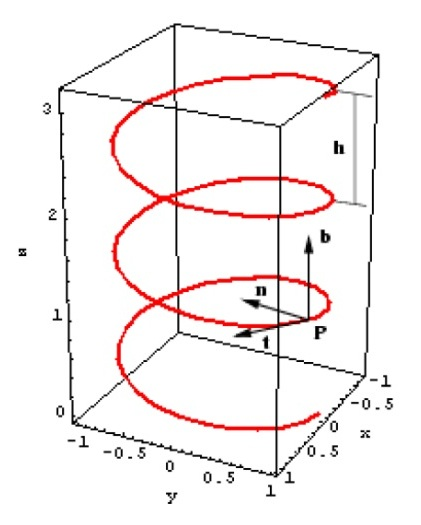
\includegraphics[width=0.5\linewidth,keepaspectratio]{ejercicio1}
\end{center}

Ayuda:

\[
\mathbf{t}'=\frac{d\mathbf{x}}{ds}; \quad 
\mathbf{t}=\frac{\mathbf{t}'}{\|\mathbf{t}'\|}; \quad
\mathbf{n}'=\frac{d^2\mathbf{x}}{ds^2}-\left(\frac{d^2\mathbf{x}}{ds^2}\bullet\mathbf{t}\right)\mathbf{t}; \quad
\mathbf{n}=\frac{\mathbf{n}'}{\|\mathbf{n}'\|}; \quad
\mathbf{b}=\mathbf{t}\times\mathbf{n}
\]

\dotfill

\[
k=\frac{r}{r+\frac{h}{2\pi}};\quad v=constante
\]

\[
T=f(s);\quad x^*(T)=x^*(f(s))=X(s);\quad \mathbf{v}=\frac{dx^*}{dt}=\frac{dX(s)}{ds}\cdot\frac{ds}{dT}=\mathbf{t}v
\]

\[
\frac{d\mathbf{v}}{dt}=\frac{d}{dt}\cdot(v\mathbf{t})=\frac{dv}{dT}t+v\frac{dt}{dT}=vk\mathbf{n}=v\frac{r}{r+\frac{h}{2\pi}}\mathbf{n}
\]

\[
T_{v}=\frac{2\pi r}{a};\quad h=T_{v}w=\frac{2\pi r}{u}w\implies w=\frac{hu}{2\pi r}
\]

\[
v=\sqrt{w^2+u^2}=\sqrt{\left(\frac{hu}{2\pi r}\right)^{2}+u^2}=\sqrt{\left(\frac{h}{2\pi r}\right)^{2}+1}\cdot u
\]

\section*{Ejercicio 2}

Probar que:

\begin{itemize}
\item $\delta_{ii}=3$

\begin{quote}
$\delta_{ii}=\sum_{i=1}^{3}\delta_{ii}=\delta_{11}+\delta_{22}+\delta_{33};
\hfill\textit{Por la definición del Delta de Kronecker.}\\
=1+1+1=3$
\end{quote}

\item $\delta_{ij}\delta_{ij}=3$

\begin{quote}
$\delta_{ij}\delta_{ij};\quad\mathbf{I}=\mathbf{I^{T}}\implies\delta_{ij}=\delta_{ji}\\=\delta_{ij}\delta_{ji};\hfill\textit{Por contracción de índices repetidos.}\\
\delta_{ii}=\sum_{i=1}^{3}\delta_{ii}=\delta_{11}+\delta_{22}+\delta_{33};\hfill\textit{Por definición del delta de Kronecker.}\\
=1+1+1=3$

No importa qué índice se utilice, el resultado será el mismo:

$\delta_{ij}\delta_{ij};\quad\mathbf{I}=\mathbf{I^{T}}\implies\delta_{ij}=\delta_{ji}\\=\delta_{ji}\delta_{ij};\hfill\textit{Por contracción de índices repetidos.}\\
\delta_{jj}=\sum_{i=1}^{3}\delta_{jj}=\delta_{11}+\delta_{22}+\delta_{33};\hfill\textit{Por definición del delta de Kronecker.}\\
=1+1+1=3$
\end{quote}

\item $\varepsilon_{ijk}\varepsilon_{jki}=6$

\begin{quote}
$\varepsilon_{ijk}\varepsilon_{jki};\quad\varepsilon_{ijk}=\varepsilon_{kij}=\varepsilon_{jki}\\
=\varepsilon_{ijk}\varepsilon_{ijk};\hfill\textit{Por la identidad epsilon-delta}\\ \delta_{jj}\delta_{kk}-\delta_{jk}\delta_{kj}=3*3-\delta_{jj}=9-3=6$
\end{quote}

\item $\varepsilon_{ijk}A_{j}A_{k}=0$

\begin{quote}
$\varepsilon_{ijk}A_{j}A_{k};\hfill\textit{Sólo quedarán los términos donde épsilon sea distinto de cero.}\\
=\varepsilon_{123}A_{2}A_{3}+\varepsilon_{312}A_{1}A_{2}+\varepsilon_{231}A_{3}A_{1}+\varepsilon_{321}A_{2}A_{1}+\varepsilon_{132}A_{3}A_{2}+\varepsilon_{213}A_{1}A_{3}$\\
\textit{Las permutaciones cíclicas de 123 valen 1 y las permutaciones cíclicas de 321 valen -1.}\\
$=A_{2}A_{3}+A_{1}A_{2}+A_{3}A_{1}-A_{2}A_{1}-A_{3}A_{2}-A_{1}A_{3}\\
\textit{Como el producto escalar conmutativo se pueden reordenar los términos}\\
=\Ccancel[red]{A_{2}A_{3}}\Ccancel[blue]{+A_{1}A_{2}}\Ccancel[green]{+A_{3}A_{1}}\Ccancel[blue]{-A_{1}A_{2}}\Ccancel[red]{-A_{2}A_{3}}\Ccancel[green]{-A_{3}A_{1}}=0$\\

Otra forma de demostrarlo es jugar con los índices:\\

$\varepsilon_{ijk}A_{j}A_{k}=-\varepsilon_{ikj}A_{j}A_{k}=-\varepsilon_{ikj}A_{k}A_{j};\hfill j=m\\
=-\varepsilon_{ikm}A_{k}A_{m};\hfill k=j\\
=-\varepsilon_{ijm}A_{j}A_{m};\hfill m=k\\
=-\varepsilon_{ijk}A_{j}A_{k};\hfill \textit{Pasando al otro término.}\\
\implies\varepsilon_{ijk}A_{j}A_{k}+\varepsilon_{ijk}A_{j}A_{k}=0\hfill\textit{Sumando.}\\
\implies 2\varepsilon_{ijk}A_{j}A_{k}=0\hfill\textit{Pasando el 2 dividiendo.}\\
\implies\varepsilon_{ijk}A_{j}A_{k}=0$
\end{quote}

\item $\delta_{ij}\delta_{jk}=\delta_{ik}$

\begin{quote}
$\delta_{ij}\delta_{jk}=\delta_{ik};\hfill \textit{Por contracción de índices repetidos.}$
\end{quote}

\item $\delta_{ij}\varepsilon_{ijk}=0$

\begin{quote}
$\delta_{ij}\varepsilon_{ijk}=\varepsilon_{iik}=\varepsilon_{jjk}=0;$\quad\textit{Porque el símbolo de permutación es cero cuando hay índices repetidos.}
\end{quote}
\end{itemize}

\section*{Ejercicio 3}

Probar la siguiente identidad usando elementos de geometría:

\[
\mathbf{A}\times(\mathbf{B}\times\mathbf{C})=(\mathbf{A}\bullet\mathbf{C})\mathbf{B}-(\mathbf{A}\bullet\mathbf{B})\mathbf{C}
\]

\dotfill

\begin{quote}
Sea $\mathbf{A}\times(\mathbf{B}\times\mathbf{C})=\mathbf{W}$ y $(\mathbf{B}\times\mathbf{C})=\mathbf{D}\implies\mathbf{D}\perp\mathbf{B};\quad\mathbf{D}\perp\mathbf{C}\\
(\mathbf{A}\times\mathbf{D})\perp\mathbf{A};\quad(\mathbf{A}\times\mathbf{D})\perp(\mathbf{B}\times\mathbf{C})\implies\mathbf{W}\text{ está en el plano $\mathbf{B}$ y $\mathbf{C}$.}$\\
Cualquier vector en el plano de $\mathbf{B}$ y $\mathbf{C}$ puede expresarse como una combinación lineal de $\mathbf{B}$ y $\mathbf{C}$.\\
$\mathbf{W}=\alpha_{1}\mathbf{B}+\alpha_{2}\mathbf{C};\quad\alpha_{1}=f(\mathbf{A},\mathbf{C});\quad\alpha_{2}=f(\mathbf{A},\mathbf{B})$\\
$\mathbf{W}$ es una función lineal de $\mathbf{A}$, $\mathbf{B}$ y $\mathbf{C}$.\\
$\alpha_{1}$ es una función lineal de $\mathbf{A}$ y $\mathbf{C}\implies\alpha_{1}=\lambda\mathbf{A}\mathbf{C}$\\
$\alpha_{2}$ es una función lineal de $\mathbf{A}$ y $\mathbf{B}\implies\alpha_{2}=\mu\mathbf{A}\mathbf{C}$\\
$\mathbf{W}=\lambda(\mathbf{A}\mathbf{C})\mathbf{B}+\mu(\mathbf{A}\mathbf{B})\mathbf{C};\hfill\textit{Le damos valores particulares a $\mathbf{A}$, $\mathbf{B}$ y $\mathbf{C}$.}$\\
$\mathbf{A}=\mathbf{B}=\mathbf{i};\quad\mathbf{C}=\mathbf{j};\quad\mathbf{W}=\mathbf{i}\times\mathbf{i}\times\mathbf{j}=\mathbf{i}\times\mathbf{k}=-\mathbf{j}$\\
$\mathbf{A}\mathbf{C}=0;\quad\mathbf{A}\mathbf{B}=\mathbf{i}.\mathbf{i}=1;\quad-\mathbf{j}=\lambda 0\mathbf{i}+\mu 1\mathbf{j}\implies\mu=-1$\\
$\mathbf{A}=\mathbf{C}=\mathbf{j};\quad\mathbf{B}=\mathbf{i};\quad\mathbf{W}=\mathbf{j}\times\mathbf{i}\times\mathbf{j}=\mathbf{i}$\\
$\mathbf{A}\mathbf{C}=1;\quad\mathbf{A}\mathbf{B}=\mathbf{j}.\mathbf{i}=0;\quad-\mathbf{j}=\lambda 1\mathbf{i}-\mu 1\mathbf{j}\implies\lambda=1$
\end{quote}

\section*{Ejercicio 4}

Probar el ejercicio anterior usando notación indicial.

\dotfill

\begin{quote}
Sea $\mathbf{B}\times\mathbf{C}=\mathbf{D}\implies\left[\mathbf{A}\times(\mathbf{B}\times\mathbf{C})\right]_{i}=[\mathbf{A}\times\mathbf{D}]_{i}\\
=\varepsilon_{ijk}A_{j}D_{k}=\varepsilon_{ijk}A_{j}\varepsilon_{kem}B_{e}C_{m}\hfill\textit{Reordenando.}\\
=\varepsilon_{ijk}\varepsilon_{kem}A_{j}B_{e}C_{m}\hfill\textit{Permutando el primer épsilon.}\\
=\varepsilon_{kij}\varepsilon_{kem}A_{j}B_{e}C_{m}\hfill\textit{Por la identidad épsilon-delta.}\\
=(\delta_{ie}\delta_{jm}-\delta_{im}\delta_{je})A_{j}B_{e}C_{m}\hfill\textit{Distribuyendo.}\\
=\delta_{ie}\delta_{jm}A_{j}B_{e}C_{m}-\delta_{im}\delta_{je}A_{j}B_{e}C_{m}\hfill\textit{Reduciendo índices.}\\
=A_{j}B_{i}C_{j}-A_{j}B_{j}C_{i}\hfill\textit{Reordenando.}\\
=(A_{j}C_{j})B_{i}-(A_{j}B_{j})C_{i}\hfill\textit{Pasando a vectorial.}\\
=(\mathbf{A}\mathbf{C})_{j}B_{i}-(\mathbf{A}\mathbf{B})_{j}C_{i}
=[(\mathbf{A}\bullet\mathbf{C})\mathbf{B}-(\mathbf{A}\bullet\mathbf{B})\mathbf{C}]_{i}$
\end{quote}

\section*{Ejercicio 5}

Probar que si $A_{\alpha_{1}\dots\alpha_{R}}$ y $B_{\alpha_{1}\dots\alpha_{R}}$ son dos tensores de orden $R$, la ecuación

\[
A_{\alpha_{1}\dots\alpha_{R}}(x_{1},x_{2},\dots,x_{n})=B_{\alpha_{1}\dots\alpha_{R}}(x_{1},x_{2},\dots,x_{n})
\]

es una ecuación tensorial; y por ello \textit{si es válida en un sistema de coordenadas cartesianas lo es en cualquier sistema de coordenadas cartesianas}.

\dotfill

\begin{quote}
$\textit{Multiplicando ambos lados por $\beta_{i\alpha_{1}\dots k\alpha_{R}}$}:\\
\beta_{i\alpha_{1}\dots k\alpha_{R}}A_{\alpha_{1}\dots\alpha_{R}}(x_{1},x_{2},\dots,x_{n})=\beta_{i\alpha_{1}\dots k\alpha_{R}}B_{\alpha_{1}\dots\alpha_{R}}(x_{1},x_{2},\dots,x_{n})\\
\implies \overline{A}_{i\dots k}(\overline{x}_{1},\dots,\overline{x}_{n})=\overline{B}_{i\dots k}(\overline{x}_{1},\dots,\overline{x}_{n})$
\end{quote}

\section*{Ejercicio 6}

Probar usando notación indicial que la contracción de dos índices cualesquiera de un 
tensor Cartesiano de orden n es un tensor cartesiano de orden $n-2$. 

\dotfill

\begin{quote}
$\overline{A}_{ijk\dots n}(\overline{x}_{1},\overline{x}_{2},\dots,\overline{x}_{n})=\beta_{i\alpha_{1}}\beta_{j\alpha_{2}}\beta_{k\alpha_{3}}\dots \beta_{n\alpha_{R}}A_{\alpha_{1}\alpha_{2}\alpha_{3}\dots\alpha_{R}}(x_{1},x_{2},\dots,x_{n})\\
\overline{A}_{iik\dots n}(\overline{x}_{1},\overline{x}_{2},\dots,\overline{x}_{n})=\beta_{i\alpha_{1}}\beta_{i\alpha_{2}}\beta_{k\alpha_{3}}\dots \beta_{n\alpha_{R}}A_{\alpha_{1}\alpha_{2}\alpha_{3}\dots\alpha_{R}}(x_{1},x_{2},\dots,x_{n})\\
\overline{A}_{ik\dots n}(\overline{x}_{1},\overline{x}_{2},\dots,\overline{x}_{n})=\delta_{\alpha1\alpha2}\beta_{k\alpha_{3}}\dots \beta_{n\alpha_{R}}A_{\alpha_{1}\alpha_{2}\alpha_{3}\dots\alpha_{R}}(x_{1},x_{2},\dots,x_{n})$
\end{quote}

\section*{Ejercicio 7}

Probar (usando notación indicial) que si $\mathbf{A}_{ij}$ es un tensor de rango 2, $\mathbf{A}_{ii}$ es un escalar. 

\dotfill

\begin{quote}
$A_{ij}\textit{ :Es un tensor cartesiano de rango 2}\\
\implies A_{ii}\textit{ :Es un tensor cartesiano de rango 0}$

$\overline{A_{ij}}=\beta_{ie}\beta_{jm}A_{em}\implies\overline{A_{ii}}=\beta_{ie}\beta_{im}A_{em};\hfill\beta\textit{ es una matriz ortogonal: }\beta^{T}=\beta^{-1}\\
(\beta_{ie}^{T}\beta_{im}=\beta_{ei}\beta_{im}=\beta^{-1}\beta=\mathbf{I}=\delta_{em})\\
=\delta_{em}A_{em}=A_{ee}=A_{mm}$
\end{quote}

\section*{Ejercicio 8}

Siendo $\mathbf{a}$, $\mathbf{b}$, $\mathbf{c}$ y $\mathbf{d}$ vectores, usar notación indicial para probar: 

\begin{itemize}
\item $\mathbf{a}\times\mathbf{b}=-\mathbf{b}\times\mathbf{a}$
\begin{quote}
$[\mathbf{a}\times\mathbf{b}]_{i}=\varepsilon_{ijk}a_{j}b_{k}\hfill\textit{Intercambiando j y k.}\\
=-\varepsilon_{ikj}a_{j}b_{k}\hfill\textit{Reordenando.}\\
=-\varepsilon_{ikj}b_{k}a_{j}=[-\mathbf{b}\times\mathbf{a}]_{i}$
\end{quote}
\item $\mathbf{a}\bullet\left(\mathbf{b}\times\mathbf{c}\right)=\mathbf{b}\bullet\left(\mathbf{c}\times\mathbf{a}\right)=\mathbf{c}\bullet\left(\mathbf{a}\times\mathbf{b}\right)$
\begin{quote}
$[\mathbf{a}\bullet\left(\mathbf{b}\times\mathbf{c}\right)]_{i}=a_{i}(\mathbf{b}\times\mathbf{c})_{i}=a_{i}\varepsilon_{ijk}b_{j}c_{k}\hfill\textit{Rotando los índices hacia la derecha.}\\
=a_{i}\varepsilon_{kij}b_{j}c_{k}\hfill\textit{Reordenando.}\\
=c_{k}\varepsilon_{kij}a_{i}b_{j}=c_{k}(\mathbf{a}\times\mathbf{b})_{k}=[\mathbf{c}\bullet(\mathbf{a}\times\mathbf{b})]_{k}$\\ \\
$[\mathbf{a}\bullet\left(\mathbf{b}\times\mathbf{c}\right)]_{i}=a_{i}(\mathbf{b}\times\mathbf{c})_{i}=a_{i}\varepsilon_{jki}b_{j}c_{k}\hfill\textit{Rotando los índices hacia la izquierda.}\\
=a_{i}\varepsilon_{jki}b_{j}c_{k}\hfill\textit{Reordenando.}\\
=b_{j}\varepsilon_{jki}c_{k}a_{i}=b_{j}(\mathbf{c}\times\mathbf{a})_{j}=[\mathbf{b}\bullet(\mathbf{c}\times\mathbf{a})]_{j}$
\end{quote}
\item $\mathbf{a}\bullet\left(\mathbf{b}\times\mathbf{a}\right)=0$
\begin{quote}
$[\mathbf{a}\bullet(\mathbf{b}\times\mathbf{a})]_{i}=a_{i}(\mathbf{b}\times\mathbf{a})_{i}=a_{i}\varepsilon_{ijk}b_{j}a_{k}\hfill\textit{Rotando los índices hacia la izquierda.}\\
=a_{i}\varepsilon_{jki}b_{j}a_{k}\hfill\textit{Reordenando.}\\
=b_{j}\varepsilon_{jki}a_{k}a_{i}=b_{j}(\mathbf{a}\times\mathbf{a})_{j}=[\mathbf{b}\bullet(\mathbf{a}\times\mathbf{a})]_{j}=[\mathbf{b}\bullet\mathbf{0}]_{j}=0;\hfill\mathbf{a}\times\mathbf{a}=\mathbf{0}$
\end{quote}
\item $\left(\mathbf{c}\times\mathbf{d}\right)\bullet\left(\mathbf{a}\times\mathbf{b}\right)=\left(\mathbf{c}\bullet\mathbf{a}\right)\left(\mathbf{d}\bullet\mathbf{b}\right)-\left(\mathbf{c}\bullet\mathbf{b}\right)\left(\mathbf{d}\bullet\mathbf{a}\right)$
\begin{quote}
$[(\mathbf{c}\times\mathbf{d})\bullet(\mathbf{a}\times\mathbf{b})]_{i}=(\mathbf{c}\times\mathbf{d})_{i}(\mathbf{a}\times\mathbf{b})_{i}=\varepsilon_{ijk}c_{j}d_{k}\varepsilon_{iem}a_{e}b_{m}\hfill\textit{Reordenando.}\\
=\varepsilon_{ijk}\varepsilon_{iem}a_{e}b_{m}c_{j}d_{k}\hfill\textit{Por la identidad épsilon-delta.}\\
=(\delta_{je}\delta_{km}-\delta_{jm}\delta_{ke})a_{e}b_{m}c_{j}d_{k}\hfill\textit{Distribuyendo.}\\
=\delta_{je}\delta_{km}a_{e}b_{m}c_{j}d_{k}-\delta_{jm}\delta_{ke}a_{e}b_{m}c_{j}d_{k}\hfill\textit{Reduciendo índices.}\\
=a_{j}b_{k}c_{j}d_{k}-a_{k}b_{j}c_{j}d_{k}\hfill\textit{Reordenando.}\\
=a_{j}c_{j}b_{k}d_{k}-a_{k}d_{k}b_{j}c_{j}=(\mathbf{a\bullet c})_{j}(\mathbf{b\bullet d})_{k}-(\mathbf{a\bullet d})_{k}(\mathbf{b\bullet c})_{j}$
\end{quote}
\end{itemize}

\section*{Ejercicio 9}

Sea $\mathbf{r}$ un radio vector y $r$ su magnitud. Probar usando notación indicial (siendo $n$ un número entero):

\begin{quote}
\hrulefill

Consideraciones:
\[
[\mathbf{r}]_{i}=r_{i}=x_{i};\quad r=\|\mathbf{r}\|=\sqrt{r_{1}^2+r_{2}^2+r_{2}^2}\implies r^2=r_{i}r_{i}=x_{i}x_{i}
\]
\[
\frac{\partial x_{i}}{\partial x_{j}}=\frac{\partial x_{j}}{\partial x_{i}}=\delta_{ij}=\delta_{ji};\quad\frac{\partial x_{i}}{\partial x_{i}}=\frac{\partial x_{j}}{\partial x_{j}}=\delta_{ii}=\delta_{jj}=3
\]
\hrulefill\\
\end{quote}
\begin{itemize}
\item $\nabla\bullet\left(r^n\mathbf{r}\right)=\left(n+3\right)r^n$
\begin{quote}
$\nabla\bullet\left(r^n\mathbf{r}\right)=\frac{\partial(r^{n}\mathbf{r})_{i}}{\partial x_{i}}=\frac{\partial(r^{n}r_{i})}{\partial x_{i}}=
{\color{red}\mathcircled{\frac{\partial r^{n}}{\partial x_{i}}}}
r_{i}+r^{n}
{\color{violet}\mathcircled{\frac{\partial r_{i}}{\partial x_{i}}}}=
{\color{red}nr^{n-2}x_{i}}r_{i}+r^{n}
{\color{violet}\delta_{ii}}\\
=nr^{n-2}x_{i}x_{i}+3r^{n}=nr^{n-2}r^{2}+3r^{n}=nr^{n}+3r^{n}=(n+3)r^{n}$\\

${\color{red} \frac{\partial r^{n}}{\partial x_{i}}=nr^{n-1}{\color{blue}\mathcircled{\frac{\partial r}{\partial x_{i}}}}=nr^{n-1}
{\color{blue}\frac{x_{i}}{r}}=nr^{n-1}n^{-1}x_{i}=nr^{n-2}x_{i}}$\\

${\color{blue}\frac{\partial r}{\partial x_{i}}=\frac{\partial \left((x_{j}x_{j})^{\frac{1}{2}}\right)}{\partial x_{i}}=\frac{1}{2}(x_{j}x_{j})^{-\frac{1}{2}}{\color{gray}\mathcircled{\frac{\partial(x_{j}x_{j})}{\partial x_{i}}}}=\frac{1}{2}(x_{j}x_{j})^{-\frac{1}{2}}
{\color{gray}2x_{i}}=\frac{1}{\sqrt{(x_{j}x_{j})}}x_{i}=\frac{x_{i}}{r}}$\\

${\color{gray} \frac{\partial(x_{j}x_{j})}{\partial x_{i}}=\frac{\partial x_{j}}{\partial x_{i}}x_{j}+x_{j}\frac{\partial x_{j}}{\partial x_{i}}=\delta_{ij}x_{j}+x_{j}\delta_{ij}=2\delta_{ij}x_{j}=2x_{i}}$\\

${\color{violet}\frac{\partial r_{i}}{\partial x_{i}}=\frac{\partial x_{i}}{\partial x_{i}}=\delta_{ii}}$\\
\end{quote}
\item $\nabla\times\left(r^n\mathbf{r}\right)=\mathbf{0}$
\begin{quote}
$\nabla\times(r^n\mathbf{r})=\varepsilon_{ijk}\frac{\partial(r^{n}\mathbf{r})_{k}}{\partial x_{j}}=\varepsilon_{ijk}\frac{\partial(r^{n}r_{k})}{\partial x_{j}}
=\varepsilon_{ijk}\left({\color{red}\mathcircled{\frac{\partial r^{n}}{\partial x_{j}}}}r_{k}+r^{n}
{\color{violet}\mathcircled{\frac{\partial r_{k}}{\partial x_{j}}}}\right)\\
=\varepsilon_{ijk}({\color{red}nr^{n-2}x_{j}}r_{k}+r^{n}
{\color{violet}\delta_{jk}})=\varepsilon_{ijk}(nr^{n-2}x_{j}x_{k}+r^{n}
\delta_{jk})=\varepsilon_{ijk}nr^{n-2}x_{j}x_{k}+\varepsilon_{ijk}r^{n}
\delta_{jk}\\
=nr^{n-2}\varepsilon_{ijk}x_{j}x_{k}+r^{n}\varepsilon_{ijk}\delta_{jk}=nr^{n-2}[\mathbf{x}\times\mathbf{x}]_{i}+r^{n}\varepsilon_{ikk}=nr^{n-2}\cdot\mathbf{0}+r^{n}\cdot 0=\mathbf{0}$\\

${\color{red} \frac{\partial r^{n}}{\partial x_{j}}=nr^{n-1}
{\color{blue}\mathcircled{\frac{\partial r}{\partial x_{j}}}}=nr^{n-1}
{\color{blue}\frac{x_{j}}{r}}=nr^{n-1}n^{-1}x_{j}=nr^{n-2}x_{j}}$\\

${\color{blue}\frac{\partial r}{\partial x_{j}}=\frac{\partial \left((x_{i}x_{i})^{\frac{1}{2}}\right)}{\partial x_{j}}=\frac{1}{2}(x_{j}x_{j})^{-\frac{1}{2}}
{\color{gray}\mathcircled{\frac{\partial(x_{i}x_{i})}{\partial x_{j}}}}=\frac{1}{2}(x_{i}x_{i})^{-\frac{1}{2}}
{\color{gray}2x_{j}}=\frac{1}{\sqrt{(x_{i}x_{i})}}x_{j}=\frac{x_{j}}{r}}$\\

${\color{gray} \frac{\partial(x_{i}x_{i})}{\partial x_{j}}=\frac{\partial x_{i}}{\partial x_{j}}x_{i}+x_{i}\frac{\partial x_{i}}{\partial x_{j}}=\delta_{ij}x_{i}+x_{i}\delta_{ij}=2\delta_{ij}x_{i}=2x_{j}}$\\

${\color{violet}\frac{\partial r_{k}}{\partial x_{j}}=\frac{\partial x_{k}}{\partial x_{j}}=\delta_{jk}}$\\
\end{quote}
\item $\Delta\left(r^n\right)=n\left(n+1\right)r^{n-2}$\\
\begin{quote}
$\Delta\left(r^n\right)=\nabla\bullet\nabla(r^{n})=\nabla\bullet\frac{\partial(r^{n})_j}{\partial x_{i}}=\frac{\partial}{\partial x_{i}}\left( {\color{red}\mathcircled{\frac{\partial(r^{n})_j}{\partial x_{i}}}}\right)=\frac{\partial}{\partial x_{i}}(nr^{n-2}x_{i})\\
=n(n-2)r^{n-3}
{\color{blue}\mathcircled{\frac{\partial r}{\partial x_{i}}}}x_{i}+nr^{n-2}{\color{violet}\mathcircled{\frac{\partial x_{i}}{\partial x_{i}}}}=
n(n-2)r^{n-3}
{\color{blue}\frac{x_{i}}{r}}x_{i}+nr^{n-2}{\color{violet}\delta_{ii}}\\
=n(n-2)r^{n-3}r^{-1}x_{i}x_{i}+3nr^{n-2}=n(n-2)r^{n-4}r^{2}+3nr^{n-2}\\=n(n-2)r^{n-2}+3nr^{n-2}=(n(n-2)+3n)r^{n-2}=(n^{2}-2n+3n)r^{n-2}\\
=(n^{2}+n)r^{n-2}=n(n+1)r^{n-2}$\\

${\color{red} \frac{\partial (r^{n})_{j}}{\partial x_{i}}=nr^{n-1}{\color{blue}\mathcircled{\frac{\partial r}{\partial x_{i}}}}=nr^{n-1}
{\color{blue}\frac{x_{i}}{r}}=nr^{n-1}n^{-1}x_{i}=nr^{n-2}x_{i}}$\\

${\color{blue}\frac{\partial r}{\partial x_{i}}=\frac{\partial \left((x_{j}x_{j})^{\frac{1}{2}}\right)}{\partial x_{i}}=\frac{1}{2}(x_{j}x_{j})^{-\frac{1}{2}}{\color{gray}\mathcircled{\frac{\partial(x_{j}x_{j})}{\partial x_{i}}}}=\frac{1}{2}(x_{j}x_{j})^{-\frac{1}{2}}
{\color{gray}2x_{i}}=\frac{1}{\sqrt{(x_{j}x_{j})}}x_{i}=\frac{x_{i}}{r}}$\\

${\color{gray} \frac{\partial(x_{j}x_{j})}{\partial x_{i}}=\frac{\partial x_{j}}{\partial x_{i}}x_{j}+x_{j}\frac{\partial x_{j}}{\partial x_{i}}=\delta_{ij}x_{j}+x_{j}\delta_{ij}=2\delta_{ij}x_{j}=2x_{i}}$\\

${\color{violet}\frac{\partial x_{i}}{\partial x_{i}}=\delta_{ii}}$\\
\end{quote}
\end{itemize}

\section*{Ejercicio 10}

Usando notación indicial probar las siguientes identidades ($\phi(x_{1},x_{2},x_{3})$: función escalar; $\mathbf{u}$, $\mathbf{v}$: campos vectoriales):

\begin{itemize}

\item $\nabla\bullet\left(\nabla\phi\right)=\nabla^{2}\phi=\Delta\phi$
\begin{quote}
$\nabla\bullet(\nabla\phi)=\frac{\partial}{\partial x_{i}}\left(\nabla\phi\right)=\frac{\partial}{\partial x_{i}}\left(\frac{\partial\phi}{\partial x_{i}}\right)=\frac{\partial^{2}\phi}{\partial x_{i}^{2}}=\Delta\phi$
\end{quote}

\item $\nabla\bullet\left(\nabla\times\mathbf{u}\right)=0$
\begin{quote}
$\nabla\bullet(\nabla\times\mathbf{u})=\frac{\partial}{\partial x_{i}}\left(\nabla\times\mathbf{u}\right)=\frac{\partial}{\partial x_{i}}\left(\varepsilon_{ijk}\frac{\partial u_{k}}{\partial x_{j}}\right)\hfill\textit{Por la derivada de un producto.}\\
=\varepsilon_{ijk}\frac{\partial}{\partial x_{i}}\left(\frac{\partial u_{k}}{\partial x_{j}}\right)=\varepsilon_{ijk}\frac{\partial^{2} u_{k}}{\partial x_{i}x_{j}}=\varepsilon_{ijk}u_{k,ij}\hfill\textit{Para los épsilon distintos de cero.}\\
=\varepsilon_{123}u_{3,12}+\varepsilon_{312}u_{2,31}+\varepsilon_{231}u_{1,23}+\varepsilon_{321}u_{1,32}+\varepsilon_{213}u_{3,21}+\varepsilon_{132}u_{2,13};\hfill\textit{Remplazando.}\\
=u_{3,12}+u_{2,31}+u_{1,23}-u_{1,32}-u_{3,21}-u_{2,13};\hfill\textit{Reordenando numeradores.}\\
=\Ccancel[red]{u_{3,12}}\Ccancel[blue]{+u_{2,31}}\Ccancel[green]{+u_{1,23}}\Ccancel[blue]{-u_{2,31}}\Ccancel[green]{-u_{1,23}}\Ccancel[red]{-u_{3,12}}=0$\\

Otra forma de demostrarlo:\\

$\varepsilon_{ijk}u_{k,ij};\hfill\textit{Artilugio: }u_{k,ij}=\frac{u_{k,ij}+u_{k,ij}}{2}\\
=\varepsilon_{ijk}\frac{u_{k,ij}+u_{k,ij}}{2}=\varepsilon_{ijk}\left(\frac{u_{k,ij}}{2}+\frac{u_{k,ij}}{2}\right)\hfill\textit{Distribuyendo.}\\
=\varepsilon_{ijk}\frac{u_{k,ij}}{2}+\varepsilon_{ijk}\frac{u_{k,ij}}{2}\hfill\textit{Permutando el segundo épsilon.}\\
=\varepsilon_{ijk}\frac{u_{k,ij}}{2}-\varepsilon_{jik}\frac{u_{k,ji}}{2}=0
$
\end{quote}

\item $\nabla\times\left(\nabla\phi\right)=0$
\begin{quote}
$\nabla\times(\nabla\phi)=\varepsilon_{ijk}\frac{\partial (\nabla\phi)_{k}}{\partial x_{j}}=\varepsilon_{ijk}\frac{\partial}{\partial x_{j}}\left(\frac{\partial\phi}{\partial x_{k}}\right)=\varepsilon_{ijk}\frac{\partial^{2}\phi}{\partial x_{j}\partial x_{k}}=\varepsilon_{ijk}\phi_{,jk}=0\\
\textit{Porque $\phi$ es un escalar.}$
\end{quote}

\item $\nabla\times\left(\nabla\times\mathbf{u}\right)=\nabla\left(\nabla\bullet\mathbf{u}\right)-\Delta\mathbf{u}$
\begin{quote}
$\nabla\times(\nabla\times\mathbf{u})=\varepsilon_{ijk}\frac{\partial (\nabla\times\mathbf{u})_{k}}{\partial x_{j}}=\varepsilon_{ijk}\frac{\partial}{\partial x_{j}}\left(\varepsilon_{kem}\frac{\partial u_{m}}{\partial x_{e}}\right);\hfill\textit{Por la derivada de un producto.}\\
=\varepsilon_{ijk}\left(\varepsilon_{kem}\frac{\partial^{2}u_{m}}{\partial x_{j}\partial x_{e}}\right)=\varepsilon_{ijk}\varepsilon_{kem}u_{m,je}\hfill\textit{Permutando el primer épsilon.}\\
=\varepsilon_{kij}\varepsilon_{kem}u_{m,je}\hfill\textit{Por la identidad épsilon-delta.}\\
=(\delta_{ie}\delta_{jm}-\delta_{im}\delta_{je})u_{m,je}\hfill\textit{Distribuyendo.}\\
=\delta_{ie}\delta_{jm}u_{m,je}-\delta_{im}\delta_{je}u_{m,je}\hfill\textit{Contrayendo índices.}\\
=\delta_{jm}u_{m,ji}-\delta_{je}u_{i,je}\hfill\textit{Contrayendo índices.}\\
=
{\color{red}\mathcircled{u_{j,ji}}}-
{\color{blue}\mathcircled{u_{i,jj}}}
=\nabla\left(\nabla\bullet\mathbf{u}\right)-\Delta\mathbf{u}$\\

${\color{red} \nabla(\nabla\bullet\mathbf{u})=\frac{\partial (\nabla\bullet\mathbf{u})_{j}}{\partial x_{i}}=\frac{\partial}{\partial x_{i}}\left(\frac{\partial u_{j}}{\partial x_{j}}\right)=\frac{\partial^{2}u_{j}}{\partial x_{j}\partial x_{i}}=u_{j,ji}}$

${\color{blue} \Delta\mathbf{u}=\nabla\bullet\nabla\mathbf{u}=\frac{\partial(\nabla\mathbf{u})_{j}}{\partial x_{j}}=\frac{\partial}{\partial x_{j}}\left(\frac{\partial u_{i}}{\partial x_{j}}\right)=\frac{\partial^{2}u_{i}}{\partial x_{j}^{2}}=u_{i,jj}}$
\end{quote}

\item $\nabla\bullet\left(\phi\mathbf{u}\right)=\nabla\phi\bullet\mathbf{u}+\phi\nabla\bullet\mathbf{u}$
\begin{quote}
$\nabla\bullet\left(\phi\mathbf{u}\right)=\frac{\partial(\phi\mathbf{u})_{i}}{\partial x_{i}}=\frac{\partial(\phi u_{i})}{\partial x_{i}}\hfill\textit{Por la derivada de un producto.}\\
=\frac{\partial\phi}{\partial x_{i}}u_{i}+\phi\frac{\partial u_{i}}{\partial x_{i}}=\nabla\phi\cdot\mathbf{u}+\phi\cdot\nabla\bullet\mathbf{u}$
\end{quote}

\item $\nabla\times\left(\phi\mathbf{u}\right)=\nabla\phi\times\mathbf{u}+\phi\left(\nabla\times\mathbf{u}\right)$
\begin{quote}
$\nabla\times(\phi\mathbf{u})=\varepsilon_{ijk}\frac{\partial(\phi\mathbf{u})_{k}}{\partial x_{j}}=\varepsilon_{ijk}\frac{\partial(\phi u_{k})}{\partial x_{j}}\hfill\textit{Por la derivada de un producto.}\\
=\varepsilon_{ijk}\left(\frac{\partial\phi}{\partial x_{j}}u_{k}+\phi\frac{\partial u_{k}}{\partial x_{j}}\right)\hfill\textit{Distribuyendo.}\\
=\varepsilon_{ijk}\frac{\partial\phi}{\partial x_{j}}u_{k}+\varepsilon_{ijk}\phi\frac{\partial u_{k}}{\partial x_{j}}\hfill\textit{Reordenando.}\\
=\varepsilon_{ijk}(\nabla\phi)_{j}u_{k}+\phi\varepsilon_{ijk}\frac{\partial u_{k}}{\partial x_{j}}\hfill\textit{Producto vectorial y definición de rotacional.}\\
=(\nabla\phi)\times\mathbf{u}+\phi(\nabla\times\mathbf{u})$
\end{quote}

\item $\nabla\bullet\left(\mathbf{u}\times\mathbf{v}\right)=\mathbf{v}\bullet\left(\nabla\times\mathbf{u}\right)-\mathbf{u}\bullet\left(\nabla\times\mathbf{v}\right)$
\begin{quote}
$\nabla\bullet(\mathbf{u}\times\mathbf{v})=\frac{\partial(\mathbf{u}\times\mathbf{v})_{i}}{\partial x_{i}}=\frac{\partial}{\partial x_{i}}(\varepsilon_{ijk}u_{j}v_{k})\hfill\textit{Por la derivada de un producto.}\\
=\varepsilon_{ijk}\frac{\partial(u_{j}v_{k})}{x_{i}}=\varepsilon_{ijk}\left(\frac{\partial u_{j}}{\partial x_{i}}v_{k}+u_{j}\frac{\partial v_{k}}{\partial x_{i}}\right)\hfill\textit{Distribuyendo.}\\
=\varepsilon_{ijk}\frac{\partial u_{j}}{\partial x_{i}}v_{k}+\varepsilon_{ijk}u_{j}\frac{\partial v_{k}}{\partial x_{i}}=\varepsilon_{ijk}u_{j,i}v_{k}+\varepsilon_{ijk}u_{j}v_{k,i}\hfill\mathit{Reordenando.}\\
=v_{k}\varepsilon_{ijk}u_{j,i}+u_{j}\varepsilon_{ijk}v_{k,i}\hfill\textit{Permutando los épsilon.}\\
=v_{k}\varepsilon_{kij}u_{j,i}-u_{j}\varepsilon_{jik}v_{k,i}=\mathbf{v}(\nabla\times\mathbf{u})-\mathbf{u}(\nabla\times\mathbf{v})$
\end{quote}

\item $\nabla\times\left(\mathbf{u}\times\mathbf{v}\right)=\left(\nabla\bullet\mathbf{v}\right)\mathbf{u}-\left(\nabla\bullet\mathbf{u}\right)\mathbf{v}+\left(\mathbf{v}\bullet\nabla\right)\mathbf{u}-\left(\mathbf{u}\bullet\nabla\right)\mathbf{v}$
\begin{quote}
$\nabla\times(\mathbf{u}\times\mathbf{v})=\varepsilon_{ijk}(\mathbf{u}\times\mathbf{v})_{k,j}=\varepsilon_{ijk}(\varepsilon_{kem}u_{e}v_{m})_{k,j}\hfill\textit{Derivada de un producto.}\\
=\varepsilon_{ijk}\varepsilon_{kem}(u_{e}v_{m})_{,j}\hfill\textit{Derivada de un producto.}\\
=\varepsilon_{ijk}\varepsilon_{kem}(u_{e,j}v_{m}+u_{e}v_{m,j})\hfill\textit{Distribuyendo.}\\
=\varepsilon_{ijk}\varepsilon_{kem}u_{e,j}v_{m}+\varepsilon_{ijk}\varepsilon_{kem}u_{e}v_{m,j}\hfill\textit{Permutando el épsilon ijk a kij.}\\
=\varepsilon_{kij}\varepsilon_{kem}u_{e,j}v_{m}+\varepsilon_{kij}\varepsilon_{kem}u_{e}v_{m,j}\hfill\textit{Por la identidad épsilon-delta.}\\
=(\delta_{ie}\delta_{jm}-\delta_{im}\delta_{je})u_{e,j}v_{m}+(\delta_{ie}\delta_{jm}-\delta_{im}\delta_{je})u_{e}v_{m,j}\hfill\textit{Distribuyendo.}\\
=\delta_{ie}\delta_{jm}u_{e,j}v_{m}-\delta_{im}\delta_{je}u_{e,j}v_{m}+\delta_{ie}\delta_{jm}u_{e}v_{m,j}-\delta_{im}\delta_{je}u_{e}v_{m,j}\\
\textit{Contrayendo índices}\\
=\delta_{ie}u_{e,j}v_{j}-\delta_{im}u_{j,j}v_{m}+\delta_{ie}u_{e}v_{j,j}-\delta_{im}u_{j}v_{m,j}\hfill\textit{Contrayendo índices.}\\
=u_{i,j}v_{j}-u_{j,j}v_{i}+u_{i}v_{j,j}-u_{j}v_{i,j}=(\mathbf{v}\bullet\nabla)\mathbf{u}-(\nabla\bullet\mathbf{u})\mathbf{v}+\mathbf{u}(\nabla\bullet\mathbf{v})-\mathbf{v}(\mathbf{u}\bullet\nabla)$
\end{quote}
\end{itemize} 

\section*{Ejercicio 11}

Es sabido que las rotaciones son no-conmutativas. Por ejemplo, tome un libro, y fije un sistema de coordenadas con ejes $x$, $y$, $z$ dirigidos a lo largo de los lados del
libro. Luego, rote primero el libro 90º en torno a $y$ ; luego rótelo 90º en torno a $z$ obteniendo una cierta configuración. Si invierte el orden de rotación, verá obtiene un resultado distinto.  

La rotación de coordenadas también es no-conmutativa; en otras palabras, el producto de las matrices $\beta_{ij}$ es no-conmutativo. Demuestre esto en el caso especial análogo a la rotación del libro mencionada más arriba. Primero transforme $x$, $y$, $z$ a $x'$, $y'$, $z'$ mediante una rotación de 90º en torno al eje $y$; luego transforme $x'$, $y'$, $z'$ a $x''$, $y''$, $z''$ mediante una rotación de 90º en torno al eje $z'$. O sea:

\[
\left(\begin{matrix}
x'\\
y'\\
z'\\
\end{matrix}\right)=
\left(\begin{matrix}
0 & 0 & -1\\
0 & 1 & 0\\
1 & 0 & 0\\
\end{matrix}\right)
\left(\begin{matrix}
x\\
y\\
z\\
\end{matrix}\right);\quad
\left(\begin{matrix}
x''\\
y''\\
z''\\
\end{matrix}\right)=
\left(\begin{matrix}
0 & 1 & 0\\
-1 & 0 & 0\\
0 & 0 & 1\\
\end{matrix}\right)
\left(\begin{matrix}
x'\\
y'\\
z'\\
\end{matrix}\right)
\]
 
Obtenga la matriz de transformación de $x$, $y$, $z$ a $x''$, $y''$, $z''$. Luego invierta el orden de rotación y muestre que se logra un resultado distinto.  

\dotfill
\begin{quote}
\[
\beta_{1}=\left(\begin{matrix}
0 & 0 & -1\\
0 & 1 & 0\\
1 & 0 & 0\\
\end{matrix}\right);\quad
\beta_{2}=\left(\begin{matrix}
0 & 1 & 0\\
-1 & 0 & 0\\
0 & 0 & 1\\
\end{matrix}\right)
\]

Primer transformación:\\
$\mathbf{x'}=\beta_{1}\mathbf{x}\\
\mathbf{x''}=\beta_{2}\mathbf{x'}=\beta_{2}\beta_{1}\mathbf{x}$\\

Segunda transformación:\\
$\mathbf{x'}=\beta_{2}\mathbf{x}\\
\mathbf{x''}=\beta_{1}\mathbf{x'}=\beta_{1}\beta_{2}\mathbf{x}$\\

\[
\beta_{1}\cdot\beta_{2}=\left(\begin{matrix}
0 & 0 & -1\\
-1 & 0 & 0\\
0 & 1 & 0\\
\end{matrix}\right);\quad
\beta_{2}\cdot\beta_{1}=\left(\begin{matrix}
0 & 1 & 0\\
0 & 0 & 1\\
1 & 0 & 0\\
\end{matrix}\right)\implies\beta_{1}\cdot\beta_{2}\neq\beta_{2}\cdot\beta_{1}
\]
\end{quote}
\section*{Ejercicio 12}

Las rotaciones infinitesimales son, sin embargo, conmutativas. Demuestre esto considerando una rotación infinitesimal de un ángulo $\theta$ en torno a $y$ seguida de otra rotación infinitesimal de un ángulo $\psi$ en torno al eje $z$. Compare los resultados con el caso en que el orden de rotaciones es invertido. 

\dotfill
\begin{quote}
\[
\beta_{y}=\left(\begin{matrix}
\cos\theta & 0 & \sen\theta\\
0 & 1 & 0\\
-\sen\theta & 0 & \cos\theta\\
\end{matrix}\right);\quad
\beta_{z}=\left(\begin{matrix}
\cos\psi & -\sen\psi & 0\\
\sen\psi & \cos\psi & 0\\
0 & 0 & 1\\
\end{matrix}\right)
\]

Primer transformación:\\
$\mathbf{x'}=\beta_{y}\mathbf{x}\\
\mathbf{x''}_{1}=\beta_{z}\mathbf{x'}=\beta_{z}\beta_{y}\mathbf{x}$\\

Segunda transformación:\\
$\mathbf{x'}=\beta_{z}\mathbf{x}\\
\mathbf{x''}_{2}=\beta_{y}\mathbf{x'}=\beta_{y}\beta_{z}\mathbf{x}$\\

Los ángulos $\theta$ y $\Psi$ son infinitesimales, entonces:\\ 

$\cos(\theta)\approx 1;\quad\sin(\theta)\approx 0\\
\cos(\Psi)\approx 1;\quad\sin(\Psi)\approx 0$

\[
\beta_{y}\cdot\beta_{z}=\left(\begin{matrix}
0 & 0 & 0\\
0 & 1 & 0\\
0 & 0 & 1\\
\end{matrix}\right);\quad
\beta_{z}\cdot\beta_{y}=\left(\begin{matrix}
0 & 0 & 0\\
0 & 1 & 0\\
0 & 0 & 1\\
\end{matrix}\right)\implies\beta_{y}\cdot\beta_{z}=\beta_{z}\cdot\beta_{y}
\]

$\mathbf{x''}_{1}=\mathbf{x''}_2\implies\beta_{z}\beta_{y}\mathbf{x}=\beta_{y}\beta_{z}\mathbf{x}\implies\beta_{z}\beta_{y}=\beta_{y}\beta_{z}$
\end{quote}

\section*{Ejercicio 13}

Demostrar que para una matriz $\mathbf{A}$ de $3\times 3$, se verifica:

\[\text{det }\mathbf{A}=\varepsilon_{ijk}A_{1i}A_{2j}A_{3k}\]

\dotfill \\

d$et\left(\begin{matrix}
a_{11} & a_{12} & a_{13}\\
a_{21} & a_{22} & a_{23}\\
a_{31} & a_{32} & a_{33}\\
\end{matrix}\right)
=a_{11}(a_{22}a_{33}-a_{32}a_{23})
-a_{12}(a_{21}a_{33}-a_{31}a_{23})
+a_{13}(a_{21}a_{32}-a_{31}a_{22})\\ \\
=a_{11}a_{22}a_{33}-a_{11}a_{32}a_{23}
-a_{12}a_{21}a_{33}+a_{12}a_{31}a_{23}
+a_{13}a_{21}a_{32}-a_{13}a_{31}a_{22}\hfill\textit{Reordenando.}\\
=a_{11}a_{22}a_{33}-a_{11}a_{32}a_{23}\\
-a_{21}a_{12}a_{33}+a_{31}a_{12}a_{23}\\
+a_{21}a_{32}a_{13}-a_{31}a_{22}a_{13}$\\

Se puede apreciar que en los seis términos que quedan aparecen en el segundo subíndice los valores 1,2 y 3. Es decir, en cada término aparecen 1, 2 y 3 como segundos subíndices . Los primeros subíndices son permutaciones que varían según la fila o columna que se utiliza para calcular el determinante.\\

$=\varepsilon_{ijk}A_{i1}A_{j2}A_{k3}$ 

\section*{Apéndice}

\textbf{Delta de Kronecker:}
\[
\delta_{ij}= \left\{\begin{array}{lcl}
             1 & ; & i=j\\
             0 & ; & i\neq j \\
             \end{array}\right.
\]

\textbf{Símbolo de permutación:}
\[
\varepsilon_{ijk}= \left\{\begin{array}{rcl}
             1 & ; & ijk=123, 312, 231 \\
             -1 & ; & ijk=321, 132, 213 \\
             0 & ; & \text{en otro caso}
             \end{array}\right.
\]

\textbf{Identidad $\varepsilon-\delta$:}

\[\varepsilon_{ijk}\varepsilon_{iem}=\delta_{je}\delta_{km}-\delta_{jm}\delta_{ke}\]

\textbf{Producto escalar (producto punto, producto interno):}\textit{ Tensor de rango 0 (escalar)}

\[
\mathbf{u}\bullet\mathbf{v}=u_{i}v_{i}=\sum_{i=1}^{3}u_{i}v_{i}=u_{1}v_{1}+u_{2}v_{2}+u_{3}v_{3}
\]

\textbf{Módulo de un vector:}

\[
u^2=u_{i}u_{i}=\sum_{i=1}^{3}u_{i}u_{i}=u_{1}u_{1}+u_{2}u_{2}+u_{3}u_{3}=u_{1}^2+u_{2}^2+u_{3}^2
\]

\textbf{Producto matricial:}

\[
\mathbf{A}\mathbf{B}=\mathbf{C}\iff A_{ik}B_{kj}=C_{ij}
\]

\textbf{Producto matrix-vector:}

\[
\mathbf{A}\mathbf{x}=\mathbf{b}\iff A_{ij}x_{j}=b_{i}
\]

\textbf{Determinante de una matrix:}

\[
\text{det } \mathbf{A}=\text{det } A_{ij}=\varepsilon_{ijk}A_{i1}A_{j2}A_{k3}
\]

\textbf{Producto vectorial (producto cruz):}\textit{ Tensor de rango 1 (vector)}

\[
\mathbf{u}\times\mathbf{v}=\varepsilon_{ijk}u_{j}v_{k}\mathbf{e}_{i}\iff\left[\mathbf{u}\times\mathbf{v}\right]_{i}=\varepsilon_{ijk}u_{j}v_{k}
\]

\textbf{Derivadas:}

\[
df=\frac{\partial f}{\partial x_{1}}dx_{1}+\frac{\partial f}{\partial x_{2}}dx_{2}+\dots+\frac{\partial f}{\partial x_{n}}dx_{n}=\frac{\partial f}{\partial x_{i}}dx_{i}
\]
\[
\frac{\partial v_{i}}{\partial x_{i}}=v_{i,i};\quad
\frac{\partial v_{i}}{\partial x_{j}}=v_{i,j};\quad
\frac{\partial^{2} v_{i}}{\partial x_{i}\partial x_{j}}=v_{i,ij}=v_{i,ji}=\frac{\partial^{2} v_{i}}{\partial x_{j}\partial x_{i}};\quad
\frac{\partial^{2} v_{i}}{\partial x_{j}^{2}}=v_{i,jj}
\]

\textbf{Gradiente de un campo escalar:}\textit{ Tensor de rango 1 (vector)}

\[
\text{grad }\phi=\nabla\phi=\frac{\partial\phi}{\partial x_{i}}=\sum_{i=1}^{3}\frac{\partial\phi}{\partial x_{i}}=\frac{\partial\phi}{\partial x_{1}}+\frac{\partial\phi}{\partial x_{2}}+\frac{\partial\phi}{\partial x_{3}}
\]

\textbf{Vector gradiente:}\textit{ Tensor de rango 2 (matriz)}

\[
\text{grad }\mathbf{v}=\nabla\mathbf{v}=\frac{\partial v_{i}}{\partial x_{j}}
\]

\[
\text{Para i=1:\quad}\sum_{j=1}^{3}\frac{\partial v_{1}}{\partial x_{j}}=\frac{\partial v_{1}}{\partial x_{1}}+\frac{\partial v_{1}}{\partial x_{2}}+\frac{\partial v_{1}}{\partial x_{3}}
\]

\[
\text{Para i=2:\quad}\sum_{j=1}^{3}\frac{\partial v_{2}}{\partial x_{j}}=\frac{\partial v_{2}}{\partial x_{2}}+\frac{\partial v_{2}}{\partial x_{2}}+\frac{\partial v_{2}}{\partial x_{3}}
\]

\[
\text{Para i=3:\quad}\sum_{j=1}^{3}\frac{\partial v_{3}}{\partial x_{j}}=\frac{\partial v_{3}}{\partial x_{1}}+\frac{\partial v_{3}}{\partial x_{2}}+\frac{\partial v_{3}}{\partial x_{3}}
\]

\textbf{Divergencia:}\textit{ Tensor de rango 0 (escalar)}

\[
\text{div }\mathbf{v}=\nabla\bullet\mathbf{v}=\frac{\partial v_{i}}{\partial x_{i}}=\sum_{i=1}^{3}\frac{\partial v_{i}}{\partial x_{i}}=\frac{\partial v_{1}}{\partial x_{1}}+\frac{\partial v_{2}}{\partial x_{2}}+\frac{\partial v_{3}}{\partial x_{3}}
\]

\textbf{Rotacional:}\textit{ Tensor de rango 1 (vector)}

\[
\text{curl }\mathbf{v}=\nabla\times\mathbf{v}=\varepsilon_{ijk}\frac{\partial v_{k}}{\partial x_{j}}
\]

\[
\text{Para ijk=123, 312, 231:\quad}\varepsilon_{123}\frac{\partial v_{3}}{\partial x_{2}}+\varepsilon_{312}\frac{\partial v_{2}}{\partial x_{1}}+\varepsilon_{231}\frac{\partial v_{1}}{\partial x_{3}}
\]

\[
\text{Para ijk=321, 132, 213:\quad}\varepsilon_{321}\frac{\partial v_{1}}{\partial x_{2}}+\varepsilon_{132}\frac{\partial v_{2}}{\partial x_{3}}+\varepsilon_{213}\frac{\partial v_{3}}{\partial x_{1}}
\]

\textbf{Laplaciano:}\textit{ Tensor de rango 1 (vector)}

\[
\nabla^{2}\mathbf{v}=\nabla\bullet\nabla\mathbf{v}=\Delta\mathbf{v}=\frac{\partial}{\partial x_{i}}\left(\frac{\partial v_{j}}{\partial x_{i}}\right)=\frac{\partial v_{j}}{\partial x_{i}\partial x_{i}}
\]

\begin{thebibliography}{1}
\bibitem{MCF}
Y. C. Fung,
\emph{A First Course in Continuum Mechanics}, 
tercera edición,
PRENTICE HALL,
1994.
\end{thebibliography}

\end{document}